% Proto board generation version 1 description
% Author: Michael Mekonnen

\documentclass[12pt]{amsart}

% Packages
\usepackage[pdftex]{graphicx}
\usepackage{hyperref}

% Custom commands
% None

\title{Proto Board Generation: Version 1}

\begin{document}

\today
\maketitle

\section{Introduction}

TODO

\section{Terms}

\subsection{Circuit}

Describes a schematic circuit as would be drawn on the GUI board by a user. An example is given in Figure \ref{fig:circuit}.

\begin{figure}
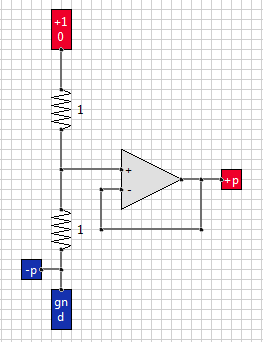
\includegraphics{Images/Circuit.png}
\caption{A voltage divider \emph{circuit}.}
\label{fig:circuit}
\end{figure}

\subsection{Circuit Piece}

(Abbreviated \emph{piece}) Describes a piece of hardware that might be put on the proto board. Examples are Op Amp packages and resistors as shown in Figure \ref{fig:pieces}.

[Related code: \url{https://github.com/mikemeko/6.01_Tools/blob/master/src/circuit_simulator/proto_board/circuit_pieces.py}]

\begin{figure}
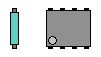
\includegraphics{Images/Circuit_Pieces.png}
\caption{Examples of \emph{circuit pieces}.}
\label{fig:pieces}
\end{figure}

\subsection{Circuit Piece Placement}

(Abbreviated \emph{placement}) Describes a placement of a number of circuit pieces on the proto board, with no wiring. An example of a placement for the voltage divider circuit shown in Figure \ref{fig:circuit} is shown in Figure \ref{fig:placement}.

\begin{figure}
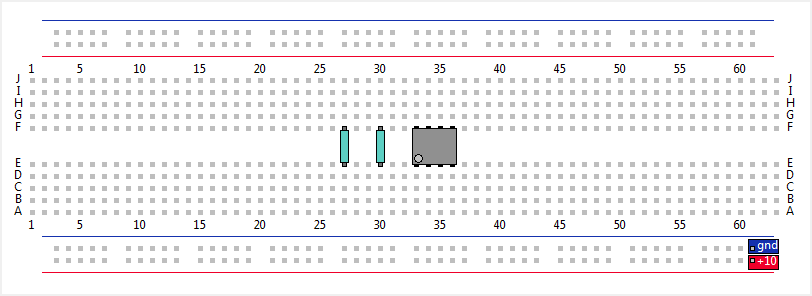
\includegraphics[width=\linewidth]{Images/Circuit_Piece_Placement.png}
\caption{\emph{Circuit piece placement} for the voltage divider circuit.}
\label{fig:placement}
\end{figure}

\section{Steps}

\subsection{Circuit to Placement}

In this first version of proto board generation from a circuit, the first step is to come up with an appropriate placement for the circuit. An example of this is the transition from Figure \ref{fig:circuit} to Figure \ref{fig:placement}. Finding a placement from a circuit involves trying various options:

\begin{enumerate}
\item There are multiple ways to package together Op Amps. For instance, if there are two Op Amps in the circuit, we can either put them together in one Op Amp piece, or we can use two Op Amp pieces (one for each Op Amp). In my solution, I try all possible ways of packaging together the Op Amps in the circuit and choose the ``best" one among all.
\item Given a set of pieces, we select a placement of the pieces on the proto board by placing the pieces on the middle strip of the proto board (connector pieces and pot pieces are handled differently, but I will ignore these pieces here for the sake of simplicity). What remains to decide now is the ordering of the pieces. The ideal thing to do is to try all possible permutations of the pieces, but this explodes quickly. My solution here is placing the pieces on the board one at a time by inserting the $k^{th}$ ($k \ge 1$) piece in the place among the $k$ possible places it can be placed while preserving the placement of the previous $k - 1$ pieces.
\end{enumerate}

Now, a natural question to ask is: how do we choose the ``best" of  set of placements? This is done by assigning a cost to each of the placements and choosing the placement with the minimum cost. The cost for a placement is evaluated by first finding all the connections that have to be made, and then computing the sum of the Manhattan distances for each of the connections.

Another natural question to ask is: how do we find the connections that need to be made on a placement? We focus on each of the nodes in the circuit, one at a time. We can find all of the points on the proto board that are a part of that node. What we need to do is put wires on the proto board so that these points are connected with one another. As the ``connections" to be made for the node, the current solution chooses pairs of these points for the node that essentially produce a minimum spanning tree of the graph of points, where the distance between two points is simply the Manhattan distance. This is done for each of the nodes in the circuit to produce one large collection of connections to make.

[Related code: \url{https://github.com/mikemeko/6.01_Tools/blob/master/src/circuit_simulator/proto_board/circuit_to_circuit_pieces.py}, \url{https://github.com/mikemeko/6.01_Tools/blob/master/src/circuit_simulator/proto_board/circuit_piece_placement.py}]

\subsection{Placement to Wired Proto Board}

Once an appropriate placement is chosen, we carry out the wiring. We do this by connecting one pair of points on the proto board at a time. While there are pairs of points remaining in the list of pairs of points to connect, we apply the following steps:

\begin{enumerate}
\item Condense: we go through the list of pairs of points and we try to replace it by another (equivalent) pair of points that are closer together.
\item Pick next pair: we then chose the next pair of points to connect. We chose the pair of points that are farthest away from each other. This decision was reached experimentally. One explanation for why this strategy seems to work best is that the farthest away pairs of points are in a way the hardest, so it is best to handle them early while there is more space on the proto board.
\item Connect: once a pair of points is chosen, the pair is connected by wires. This is done by a search mechanism with various heuristics that favor quickly finding a wiring and making the resulting wiring aesthetically pleasing.

[Related code: \url{https://github.com/mikemeko/6.01_Tools/blob/master/src/circuit_simulator/proto_board/find_proto_board_wiring.py}]
\end{enumerate}

An example of a wired proto board is given in Figure \ref{fig:wired}.

\begin{figure}
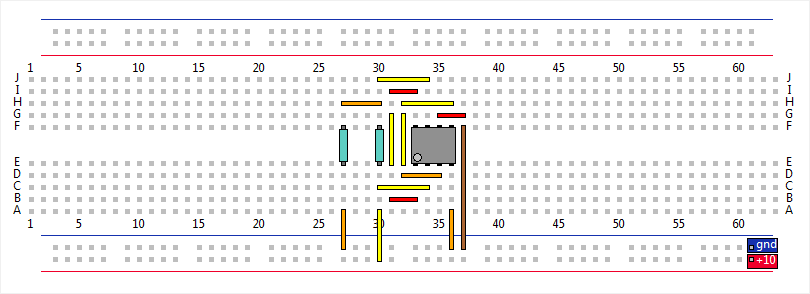
\includegraphics[width=\linewidth]{Images/Wired_Proto_Board.png}
\caption{A wired proto board for the voltage divider circuit.}
\label{fig:wired}
\end{figure}

\end{document}
